\chapter{Module: Core-Framework}
\label{ch:core}

\section{Network}
The network implementation uses the concept of \emph{leechers} and \emph{seeders}. A leecher connects to one or more seeders and downloads chunks from them. A seeder has multiple leechers connected to it and uploads chunks to them. Chunk transfers are pull-based, so they can only be requested by the leecher, while meta data or address announcements are push-based and thus transferred without being requested. Therefore, every leecher knows exactly what a seeder has to offer without asking, but only requests the chunks it needs. See section \ref{subsec:downloadreq} for more information.

While leechers and seeders are independent of each other, it is possible to couple them together. A leecher coupled with a seeder always announces the address of its seeder to any other seeder it is connected with. This concept is explained in more detail in section \ref{subsec:autoconnect}.

Both, a leecher and a seeder, keep a reference to a database instance. A leecher stores downloaded data in its database and a seeder uploads data from its database. It is possible that both reference the same database instance, so the seeder is able to upload data, which was downloaded by the leecher. The DataBase module and all related concepts are explained in chapter \ref{ch:database}.

Leechers and seeders are associated with one of the multiple distribution algorithms defined in the Algorithm module. These algorithms determine the distribution behavior, which is further described in chapter \ref{ch:algorithm}.


\subsection{Automatic Connect}
\label{subsec:autoconnect}

\begin{figure}[ht]
	\centering
	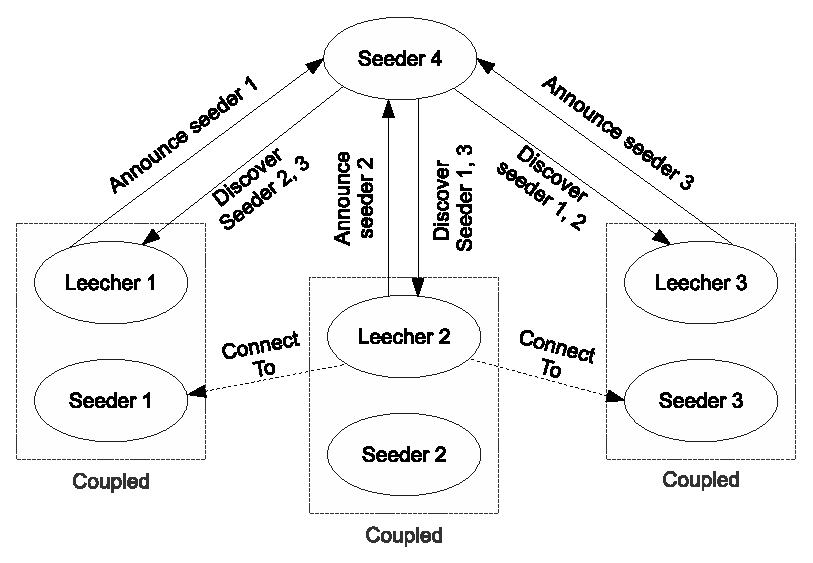
\includegraphics[width=0.6\linewidth]{autoconnect}
	\caption{Seeder Discovery}
	\label{fig:autoconnect}
\end{figure}

\begin{figure} [ht]
	\centering
	\begin{minipage}[b]{0.6\linewidth}
		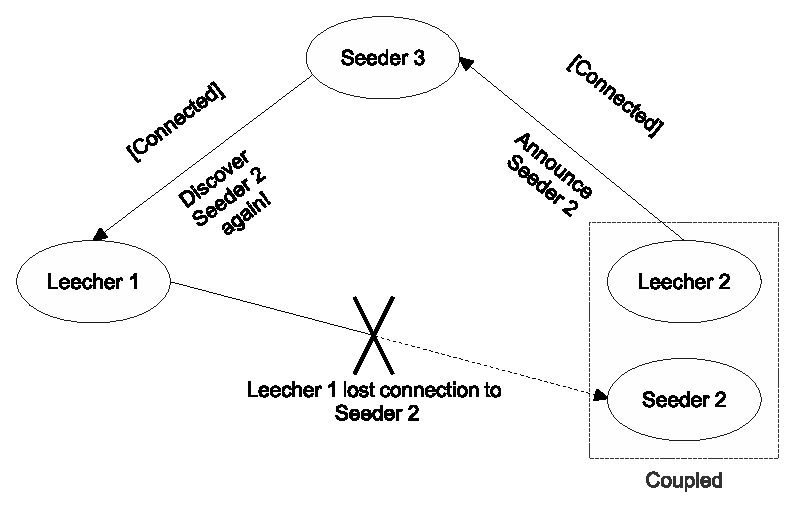
\includegraphics[width=\textwidth]{reconnect}
		\caption{Reconnect}
		\label{fig:reconnect}
	\end{minipage}
	\hspace{0.1\linewidth}
	\begin{minipage}[b]{0.25\linewidth}
		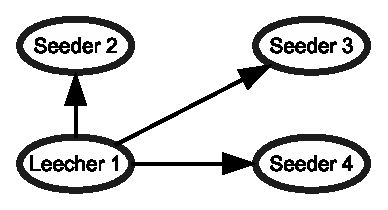
\includegraphics[width=\textwidth]{mesh}
		\caption{Leecher\,/\,Seeder mesh}
		\label{fig:mesh}
	\end{minipage}
\end{figure}

Figure 5.1 shows in detail how the automatic connect mechanism works. Every leecher has to manually connect to a seeder for the first time, thereafter a leecher is able to automatically connect to other seeders. In order to provide this functionality every leecher, who is coupled with a seeder, announces the address of its coupled seeder to all other seeders it is currently connected with.

In this scenario leechers one, two and three announce the addresses of their seeders to seeder four, which broadcasts these addresses to all connected leechers. This way the leechers get to know each other and can connect to the remaining seeders. In figure \ref{fig:autoconnect} only the new connections of leecher two are illustrated, though leecher one and three connect to the other seeders as well. This works recursively, so if one of the seeders already has other leechers connected to it, these also will be found. Finally, the topology is just a mesh with $(n\:-\:1)\cdot n$ connections, where $n$ refers to the total number of coupled seeders and leechers and every leecher of each couple is connected to every seeder of all other couples. Figure \ref{fig:mesh} shows this from the point of view of leecher two, which is connected to all others seeders.

The mesh topology implies, that every peer knows exactly, what data sets other peers have and thus can request chunks efficiently, though it adds exponentially growing overhead and thus does not scale indefinitely. To improve scalability, the number of connections per leecher can be limited, which also limits the knowledge of each leecher and thus the ability to make good decisions what to request from whom.

If a leecher loses, for some reason, the connection to a seeder, the framework is able to reconnect, if the seeder is still online. This will be detected by periodic address broadcasts. So if, as shown in figure \ref{fig:reconnect}, leecher one lost the connection to seeder two but leecher one and two are also connected to seeder three, then seeder three will notify leecher one, that seeder two still exists.


\subsection{Meta Data Announcements}
After a leecher connected to a seeder, the leecher does not know, which data sets the seeder offers. As previously explained in section \ref{subsec:autoconnect}, leechers discover new seeders through seeders they are already connected with. The way a leecher collects knowledge about the data sets a seeder offers works in a similar way. A seeder announces periodically its data sets to all connected leechers. It basically transfers a list of meta data, which is explained further in section \ref{sec:metadata}, so every leecher can update its knowledge about this seeder. The list of meta data can be modified by the used distribution algorithm before it is announced to model a specific distribution behavior. Chapter \ref{ch:algorithm} outlines this mechanism.

An optimization uses a lazy transmission approach, thus a seeder will only transfer meta data, if it has changed. So if a data set does not change at all, a seeder will never transfer a second announcement of this data set. Another optimization causes the seeder not to transfer any announcements to leechers, which the seeder is uploading data to. This feature is further explained in the following section \ref{subsec:downloadreq}.


\subsection{Download Requests}
\label{subsec:downloadreq}
After a leecher successfully connected to one or more seeders and has already received meta data announcements, it can start to request chunks from the seeders. What to request from whom heavily depends on the used distribution algorithm, which is explained in chapter \ref{ch:algorithm} in more detail. 

Since downloading more than one chunk at a time from the same seeder is not faster than downloading them sequentially, only one download per seeder at a time is allowed, which also reduces protocol complexity. Because of that, during a chunk download meta data and address announcements are not transferred, because these are obviously of no interest for the leecher. As soon as the chunk download completes, outstanding announcements will be bundled and transferred.

A seeder is allowed to decide whether a chunk request is valid or not, which means depending on the algorithm the seeder can reject a chunk request. If a seeder rejects a chunk request the leecher will not request the same chunk again. The seeder can tell the leecher, that a previously rejected chunk request is valid again by reannouncing this specific chunk. This way complex distribution behavior
can easily be implemented.


\subsection{Nonblocking I/O}
Network communication is based on \emph{sockets}, which can either be datagram or stream based. Datagram sockets are connectionless, so they are of no importance for this thesis. Instead, the network implementation uses stream sockets. A stream socket is always connected to another socket. Programmatically, these two sockets behave like files. If data is written to a socket, it will be transferred to the other socket and can be read from it then. As with files, socket operations usually block the currently executing \emph{thread} until the requested data is read or written, so this requires one thread per socket to handle multiple sockets concurrently. Unfortunately, threads are a limited resource, because they increase memory and \emph{CPU} usage. Therefore, this concept does not scale well.

To handle multiple sockets per thread, so called \emph{nonblocking} sockets in combination with \emph{event-polling} can be used. A nonblocking socket generally does not block on an operation, but returns an error instead, if it is not ready to execute this operation immediately. In combination with event-polling a thread can listen on sockets and be notified when these are ready. With this technique a single thread can handle tens of thousands of sockets.

Unfortunately, nonblocking sockets increase the complexity significantly, so the network implementation uses a framework to simplify the usage of them. The framework is called \emph{Netty 5} and written in Java. Netty supports the separation of the transport protocol and the logic, so underlying transport protocols, like \emph{In-VM}, \emph{TCP}, \emph{SCTP} or \emph{UDT}, can be changed without affecting the logic of the application. By default, only In-VM and TCP is used, which are explained in section \ref{subsec:transport}.

\subsection{Transport: In-VM and TCP}
\label{subsec:transport}
Netty offers an In-VM, also called local, transport protocol, which does not involve network at all. It only works inside a single instance of the \emph{JVM} and is perfectly suited for simulations or benchmarking. This is because, the local transport does not require (de-)serialization of data, which eliminates a huge amount of memory and CPU usage. Normally, the overhead of serialization is negligible, but the Benchmark module is able to simulate a large number of seeders and leechers, so these overheads can sum up to a significant number. Therefore, the local transport seems to be the perfect fit for this purpose.

Netty also offers common transport protocols like TCP. It is used as a secondary option for the Benchmark module, which is useful to run distributed benchmarks on multiple machines, because local transport is limited to a single JVM instance.


\subsection{Traffic-Shaping}
In order to simulate and evaluate network applications, the ability to control the bandwidth to have comparable network conditions is needed. The problem with bandwidth limitation, which is also called traffic-shaping, is that the writer can not be throttled. The writer can either write as fast as possible or not write at all. In order to limit the bandwidth, the writer has to be started and stopped periodically. Since readers and writers are identical in terms of bandwidth limitation, the explanation always refers to writers but the same approach works for readers equally well.

If the limitation period is too long, the introduced bandwidth peaks will affect the measurements in a negative way, but if the period is too short instead, overhead will be increased. To perfectly limit the bandwidth an indefinitely short interval is needed. So, if the traffic-shaping shall work reliably the sweet spot between accuracy and minimal overhead has to be found. The network implementation uses a period of 250\,ms, which offers enough precision, because the measurements are done every second. So every measurement contains the average of approximately four bandwidth limitation runs.

The complexity increases using multiple writers, who are not allowed to exceed a shared bandwidth. The main problem is fairness. It is not desired, that one writer gets 95\,\%, while the remaining writers share only 5\,\% of the bandwidth. At the same time a single writer should be able to write at full speed, when no one else is writing. This complex behavior can be achieved using a \emph{leaky-bucket} algorithm and a \emph{priority-queue}.

A leaky-bucket contains tokens, where a token equals one byte. If a writer wants to write a message, it will try to remove the tokens needed for the message to transfer. If the bucket does not have enough tokens, the writer will take the remaining tokens and will decrease the size of the message it wants to write by the number of removed tokens. After this, the writer waits until the bucket gets refilled and repeats the procedure. Unfortunately, this does not fix the fairness problem.

To solve the fairness problem a writer is not allowed to remove tokens from the bucket directly. Instead it inserts the write request into a priority-queue. A writer job constantly polls the head of the queue and tries to process the write requests using the leaky-bucket. This time, the writer increases its number of written bytes according to the size of the written message. If the writer has more messages to write, it will insert itself into the queue according to the number of total written bytes compared to other writers. This way the head of the queue always is a write request belonging to a writer, which has written the fewest number of bytes in total. Thereby we get good fairness with almost no overhead, because the writer job runs only on demand in a thread pool and quits after all write requests are processed.

\cleardoublepage
\section{Concurrency}
With the use of nonblocking sockets it is possible to handle a lot of sockets with only one thread. But this can be further improved, because modern CPUs always have multiple cores, whose quantity determines the number of threads able to run in parallel. For example, if a CPU has four cores and the application only uses one thread, the CPU will be utilized by only 25\,\%. Wherefore Netty uses more than one thread to increase the efficiency. In the next section \ref{subsec:eventloop} the utilization of multiple threads is explained in more detail.

\subsection{Event-Loop}
\label{subsec:eventloop}
Netty has the notion of an \emph{event loop}. An event loop is always running in its own thread and processes queued events one after the other. These events are mostly readiness events notifying a given socket is now readable, writable, acceptable or connectable.

To use more than one thread, Netty simply spawns more event loops, typically just as many as there are CPU cores. New sockets will then be distributed evenly among all running event loops. Even if the event loops get unbalanced, Netty will try to rearrange the sockets so that the event loops become balanced again.

These event loops can then run theoretically in parallel, because the underlying operating system distributes busy threads equally among all available cores. But using more than one thread is only the tip of the iceberg, multiple threads introduce a whole new category of problems and considerations, which have to be taken into account. The next section \ref{subsec:lockfree} discusses this a bit more in depth.


\subsection{Lock-Free Progamming}
\label{subsec:lockfree}
The main problem using multiple threads is the question of how these threads interact which each other. If two threads access the same variable without any protection, the resulting behaviour is not always defined and can lead to untraceable bugs. The unprotected access of variables is called a \emph{race condition} or \emph{critical-section}.

A simple solution is to protect those sections with a mutually exclusive (mutex) lock, which simply forbids that more than one thread is entering the critical section at a time, but this decreases efficiency and increase thread context switching, which is expensive. One solution is to use lock-free algorithms, which exploit certain guarantees made by the Java memory model. The in-depth explanation of these concepts would arguably exceed the boundaries of this thesis, but it should be noted, that the network implementation heavily uses those algorithms.

The reason why those concepts were considered is that inter-thread communication was a key design choice in order to simplify the architecture of the implementation. For instance a leecher can be connected to a lot of seeders receiving a lot of meta data and address announcements. In order to effectively request chunks from the seeders, the leecher has to collect the information from all connections, which may run in different event loop threads and thus are not protected against concurrent access by default. Since this collection is a common task, it should be optimized as well. Using so called \emph{compare and swap (CAS)} and volatile operations the necessary mutexes can be reduced to a minimum. 

Usually, the overhead of mutexes can be ignored, but the simulation of hundreds of leechers and seeders on multiple cores means a lot of cross thread access. If every collection of meta data of each leecher would stop all event loop threads by using a mutex, the overhead should start to be noticeable. These impacts are hard to measure or quantify, though. But in principle the lock-free approach scales better. As a rule of thumb lock-free algorithms should always be preferred in performance critical sections. They can also help to prevent \emph{dead locks}, which happen when two threads are waiting for resources locked by each other, and thus both wait forever.

\cleardoublepage
\chapter{Module: DataBase}
\label{ch:database}
The DataBase module represents a generic interface for storing binary data sets as chunks in any kind of storage. It has the responsibility to verify written chunks in terms of consistency and validation. But to do so the database has to know about the structure of the data set. Therefore, the meta data, which describes a given data set, is stored together with the data set as key-value pairs. The next section \ref{sec:metadata} describes the meta data format in more detail.


\section{Meta Data}
\label{sec:metadata}
The meta data contains information about a given data set. These information are transferred between seeders and leechers to describe what data sets are available, and thus which chunks can be requested. The following information are stored in the meta data: \emph{Name}, \emph{Description}, \emph{ID}, \emph{Size}, \emph{Chunks}, \emph{Hash} and \emph{ChunkedHashes}.

The Name and Description fields are used for human related tasks. The ID is used for streaming purposes, which will be explained later in chapter \ref{ch:streaming}. The Size field determines the total size of the data set including all chunks, which leads to the next field. The Chunks field is a bit set, which simply stores one or zero bits for existing or missing chunks respectively. The length of the bit set determines the number of chunks a data set has. The Hash field contains a checksum generated by a hash algorithm like \emph{SHA-1} from the whole data set. The ChunkHashes field does the same but for each chunk individually. This way the database can verify single chunks as well as the data set in total. The reason why there is an extra Hash field for the whole data set is to reduce the chance of hash collision. Two data sets are considered equal if all of their fields are equal as well.


\section{Backends: Emulated, In-Memory and Persistent}
\label{sec:backend}
The emulated backend does not store any data sets directly. Instead, it only stores which data sets and chunks are available and thus causes no overhead at all. If data sets are queried, empty buffers are returned. The in-memory backend stores data sets in main memory and is not persistent. It is a useful backend for situations, where data sets are generated or consumed on the fly like video streaming or test scenarios. In case of video streaming, a webcam could act as a data set source and thus chunks are transmitted directly from it. This backend has almost no overhead other than memory usage. The persistent backend implements a database based on a file system, which can also be virtual like a \emph{ZIP} file. This backend is more rigid but also very important for file sharing applications.


\cleardoublepage
\chapter{Module: Algorithm}
\label{ch:algorithm}
This module contains the algorithms which determine the distribution behavior. While the Core-Framework module takes care of all the low-level parts the real work is done here. This module defines two interfaces for both, a seeder and a leecher, which are called \emph{SeederDistributionAlgorithm} and \emph{LeecherDistributionAlgorithm} respectively. 

A SeederDistributionAlgorithm can modify meta data, which is announced by a seeder and allows or rejects chunk requests. A LeecherDistributionAlgorithm is even simpler, it can only request chunks. A simplified implementation of both interfaces would look like this:

\begin{verbatim}
interface SeederDistributionAlgorithm {
    List of MetaData modifyMetaData(List of MetaData)
    Bool isChunkRequestAllowed(ChunkRequest)
}

interface LeecherDistributionAlgorithm {
    List of ChunkRequest requestChunks(AvailableDataSetsOfAllSeeders)
}
\end{verbatim}

These interfaces are totally independent of the underlying network implementation. As a core concept, a leecher algorithm is only interested in requesting chunks as efficient as possible. The seeder can decide if a requested chunk request is allowed or not and what meta data it announces. With those two methods a seeder can model the behavior of a seeder which uploads to every leecher in parallel, or only to one leecher in total, or even stop announcing meta data, if the associated data sets have already been transferred, which is used by the Chunked-Swarm model and explained in section \ref{sec:chunkedswarm}. In the next sections all implemented distribution algorithms are compared and explained in detail.

\section{Algorithms: Sequential and Logarithmic}
\label{sec:seqlog}
The Sequential and Logarithmic model, explained in section \ref{sec:sequentialmodel} and \ref{sec:logarithmicmodel} respectively, both share the same LeecherDistributionAlgorithm, which is the \emph{OrderedSingleMostLeecherDistributionAlgorithm}. This algorithm chooses a seeder, which has the complete data set and requests it from this seeder. It does only work with a chunk count of one and never requests a data set from more than one seeder in parallel.

For seeding the Sequential model uses the \emph{DefaultSeederDistributionAlgorithm}, which uploads data sets to every leecher asking for one. It is important to note, that this model has only one seeder and many leechers. All leechers are connected to this seeder and download data sets sequentially. 

The Logarithmic model is fundamentally different in this regard, because every peer has a leecher coupled with a seeder and is connected to every other seeder of the network. This model uses the \emph{LimitedSeederDistributionAlgorithm} for seeding and uploads data sets only to one leecher in parallel. During an upload other requests are rejected. The meta data of data sets which are being uploaded are also removed from the meta data announcement set, so new leechers will not request these data sets. After an upload is complete, the meta data of the particular data set is announced again.

\section{Algorithm: Chunked-Swarm}
\label{sec:chunkedswarm}
The Chunked-Swarm model allows multiple uploads in parallel and requires a chunk count equal to or greater than the number of peers. Every seeder uses the DefaultSeederDistributionAlgorithm and thus uploads chunks to every leecher. The leechers use the \emph{OrderedChunkedSwarmLeecherDistributionAlgorithm}, which is similar to the OrderedSingleMostLeecherDistributionAlgorithm, but requests single chunks instead of complete data sets and will download from any seeder the leecher is connected with in parallel, if this is possible. 

To effectively download from as many seeders as possible, all seeders are sorted by the number of chunks they offer in ascending order, but without the chunks, which are currently being downloaded by the leecher and those, which are already downloaded. The leecher then traverses the sorted list of chunks and requests one chunk from each seeder. After each request the list is sorted and filtered again, so that the chunk the leecher just requested is not requested from an other seeder as well. 

This way the leecher always chooses the best combination of chunk requests. If there are multiple chunks per seeder, which are equally well suited for downloading, the algorithm picks one chunk randomly. In consequence of this, chunk duplication cannot be prevented, though minimized if a high chunk count is chosen. Although, the efficiency of this model was determined with perfect chunk selection in mind. 

Since random chunk selection can not always be perfect, an additional so called \emph{SuperSeederDistributionAlgorithm} can be chosen. It is basically a DefaultSeederDistributionAlgorithm which remembers all chunks it has already uploaded and rejects any further attempts to download these chunks. It is typically used by only one seeder in the network, which is then called a \emph{super seeder}. This way chunk duplication cannot occur, because leechers, whose chunk requests are rejected, simply request another chunk and request the rejected chunk later from normal seeders. The method guarantees that every leecher requests a distinct chunk from the super seeder, which has the complete data set at the beginning. The other seeders still use the DefaultSeederDistributionAlgorithm. The problem is, that this technique is not safe against peer loss, which means that chunks uploaded to a peer, which goes offline, are not retransferred by the super seeder by default. This relates to future work and could be solved by periodic checks which peers are still online.

\cleardoublepage
\chapter{Modules: Monitoring, Record-Viewer and Benchmark}
\label{ch:monitoring}

To measure the quality and efficiency of the framework, the Monitoring module collects data like current bandwidth usage, total transferred bytes and chunk\,/\,data set completion timestamps from every peer. The current upload bandwidth usage and total uploaded bytes are only collected from seeders, while the current download bandwidth usage and total downloaded bytes are only collected from leechers. That is because leechers upload almost nothing, they only announce the address of their coupled seeder once and upload a chunk request for each chunk. These chunk requests are very small in terms of memory usage and usually are only transferred once every few seconds, depending on the chunk size. In consequence of that, the seeders only download those address announcements and chunk requests from their leechers, so seeders download almost nothing as well.

The collected data is then stored in csv files, which contain columns for every leecher and\,/\,or seeder, depending on the collected data. Because these files alone are not very meaningful, a small collection of python scripts helps to manage them. For instance, if there a multiple csv file sets from many runs, the merge script can calculate the mean and the confidence interval of all runs. Also, additional csv files are created from existing csv files, like the SortedTotalUploadedBandwidth.csv and SortedChunkCompletion.csv files which are, as the name let assume, sorted. In case of the SortedTotalUploadedBandwidth.csv file, the entries are sorted by the amount of uploaded bytes and the SortedChunkCompletion.file is sorted by the time needed to complete all chunks\,/\,data sets. Both files are sorted in descending order.

Besides the csv files, the Monitoring module can create a log file, which contains a chronological stream of events occurred during a run. Amongst others, these events are chunk requests, starts of uploads and downloads and chunk\,/\,data set completions. The content of the log file can be rendered using the Record-Viewer module. Those events are stored using Java serialization and could be generated by the Benchmark module or any other application, which uses the Monitoring module.

The Benchmark module consists of a command line application, which simulates a configurable number of seeders and leechers in one process and records its runtime behavior. The application can be configured in several ways to implement a wide range of scenarios and is bundled as a Java archive (\,\emph{jar}\,) file. This module uses the emulated database backend, which is explain in section \ref{sec:backend}, so there is almost no overhead involved. Chapter \ref{ch:eval} explains this module a bit more in depth during the evaluation of the distribution algorithms presented in section \ref{ch:algorithm} and chapter \ref{ch:theory}.


\chapter{Module: Streaming}
\label{ch:streaming}

The Streaming module contains an experimental implementation of a video streaming server, where peers can start watching a video file roughly at the same time and continue watching the video while they are downloading and distributing new chunks from the server. 

In order to transfer the data set to all peers contiguously, the video file has to be separated into multiple parts, which consist of multiple chunks. Programmatically, each part is represented by a data set, so there is no data set, which describes the whole video file at once. To determine which data set represents which part of the video file, the meta data of each data set contains an ID field, which is linearly incremented for each part. All data sets combined together represent the whole video file. The peers always try to download and distribute data sets with the smallest ID field. This way, the video file is distributed sequentially while retaining the efficiency of the Chunked-Swarm model.

The size of the parts have to be chosen wisely, because it determines how long it takes to distribute a part among all peers. Since peers can only start watching the video, when there is at least one part available, the size of the parts directly affects the quality of service. The correct choice of the size also depends on the number of chunks and thus on the number of peers.

The Streaming module uses an \emph{HTTP} server to deliver the data sets from the database as a video stream. Even if there is only one data set available, the HTTP server will set the content length of the HTTP response to length the of the whole video file. Therefore, external video players can simply play the whole video file at once. If the video player requests a position in the video stream which is not available yet, the HTTP server will wait until the database contains enough data sets to process the request. From the point of view of the video player it looks like the data comes in very slowly and thus waits until enough bytes have been buffered to play the video fluently.
